\section{Case studies}
\label{sec:nn-exp_case}

Here we describe our case studies developed in order to experiment with
our algorithms and to build new benchmarks for the verification community:
Adaptive Cruise Control~\cite{DBLP:conf/ecms/DemarchiGPT22} and drone
control.
The purpose of creating a new benchmark for the evaluation of verification 
algorithms is that, while the verification community has been prolific in 
developing novel methodologies, very few general benchmarks have been proposed,
among which the most popular is still the ACAS XU 
benchmark~\cite{DBLP:conf/cav/KatzBDJK17}, released in 2017.

Furthermore, autonomous driving and drone control are tasks relevant for modern
applications and, at the same time, the neural networks used in this kind of 
control are usually small enough for the existing verification methodologies 
to be successfully applied. 

\subsection{Adaptive Cruise Control}

Technically, an adaptive cruise control (ACC) is an autonomous driving
function of level one\footnote{``Taxonomy and Definitions for Terms
	Related to Driving Automation Systems for On-Road Motor Vehicles'',
	SAE Standards, J3016\_202104.}, which controls the
acceleration of the \emph{ego car} --- the car whereon the ACC is
installed --- along the longitudinal axis. An ACC has two competing
objectives: keeping 
the ego car at the speed set by the user (\textit{speed following
	mode}) and keeping a safe distance from the \emph{exo car} in front
(\textit{car following mode}). The ACC that we consider has one
output, i.e., the acceleration $a$ suggested to the ego car in
$m \cdot s^{-2}$, and five inputs, two of which are fixed:
%
\begin{itemize}
	\item $v_p [m \cdot s^{-1}]$: the speed of the ego car.
	\item $v_r [m \cdot s^{-1}]$: the speed of the exo car relative to
	the ego car; when there is no exo car, this input has the value
	$0$.  
	\item $D [m]$: the actual distance between the ego car and the exo
	car; when there is no exo car or when the exo car is farther than
	$150m$ this input has the default value of $150m$.  
	\item $TH [s]$: Minimum headway time; this is the minimum
	time gap between the exo car and the ego car: $TH \cdot
	v_p$ corresponds to $D_s$, i.e.,the \emph{minimum safety
		distance}.
	\item $D_0 [m]$: A safety margin to be added to the minimum safety
	distance $D_s$.
\end{itemize}
%
In production vehicles the ACC function is implemented using classical
control laws. We view the production function --- called $ACC_{o}$
in the following --- as a black-box whose behavior should be learned
by a neural network.

\begin{figure}[t]
	\caption{Box plot for a million samples of the Adaptive Cruise Control 
		data set ($TH = 1.5$; $D_0 = 5$)}
	\label{fig:cruise-boxplot}
	\centering
	\scalebox{0.25}{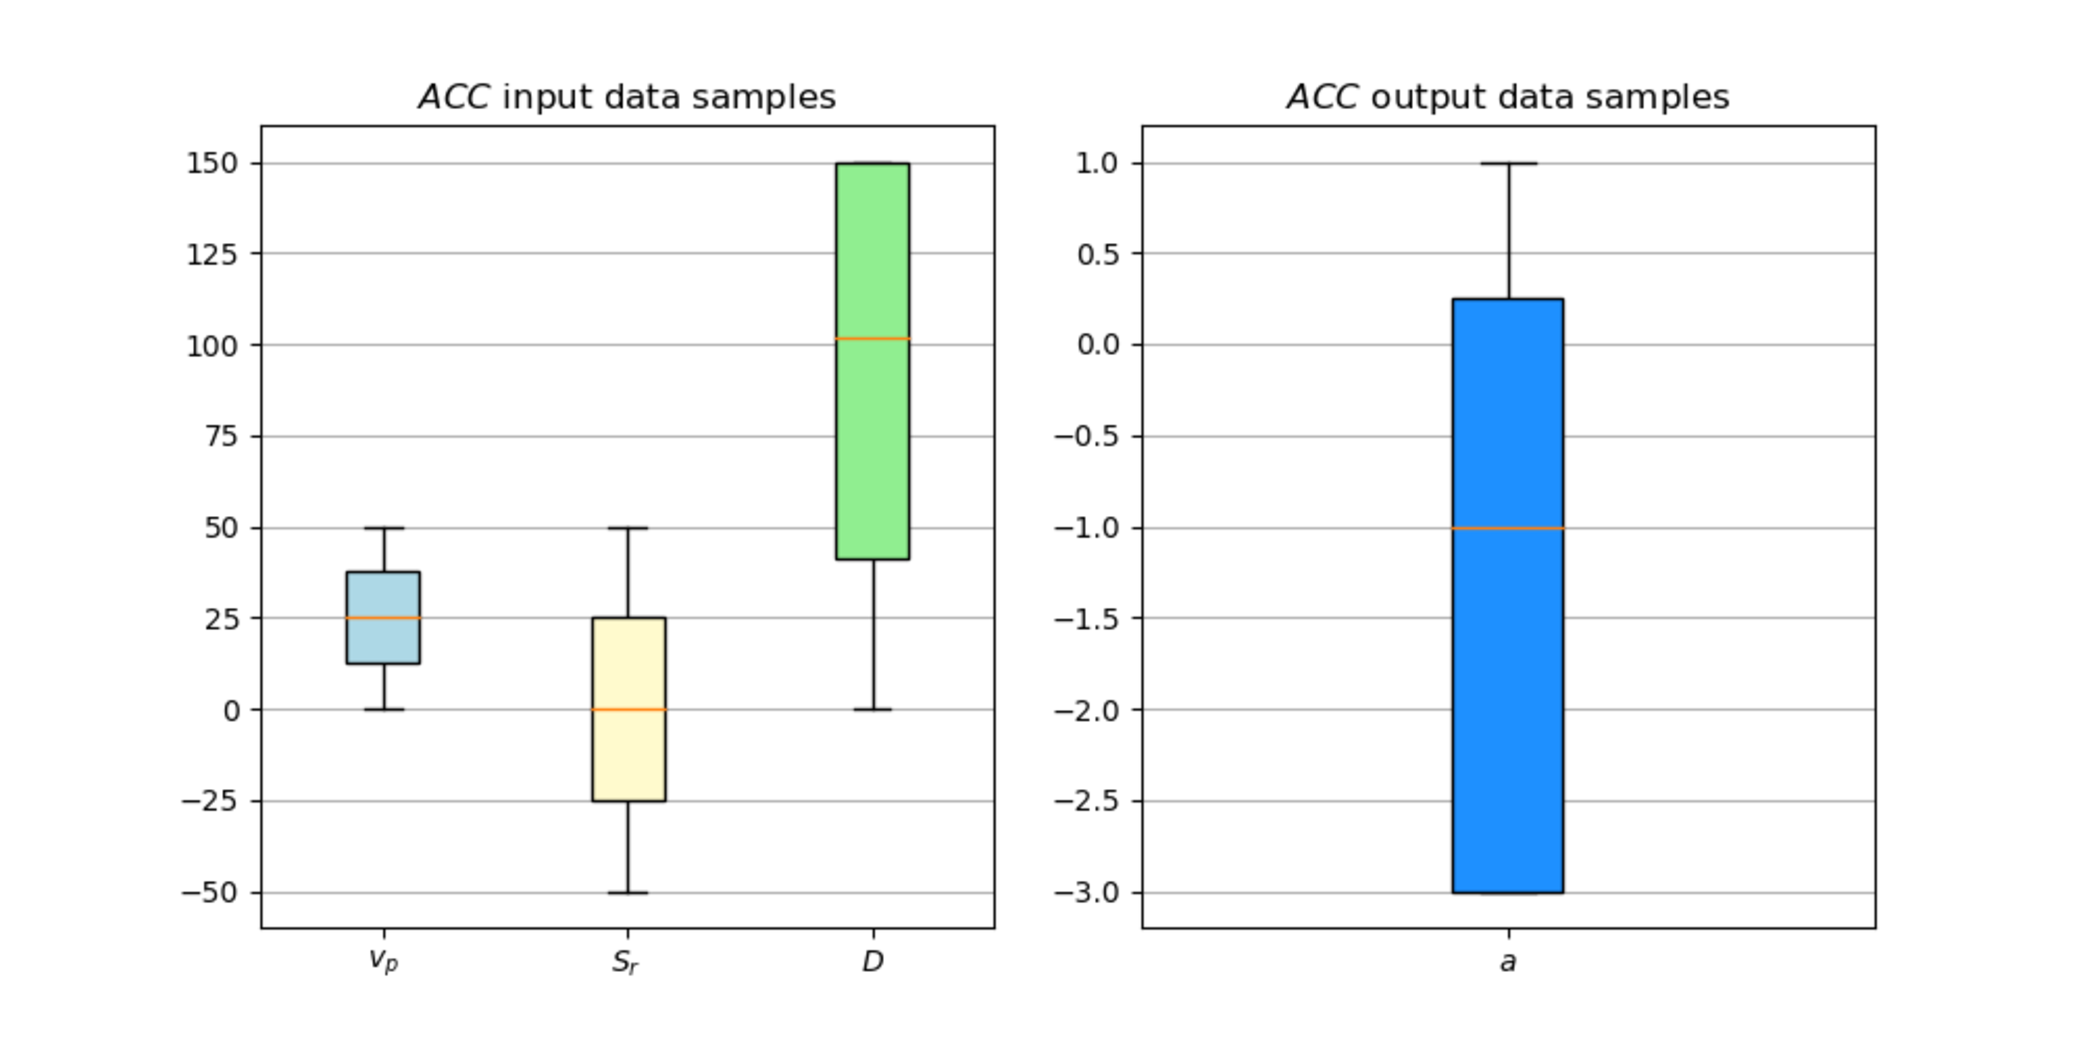
\includegraphics{NN/acc_samples.pdf}}
\end{figure}

Given the goal of learning $ACC_{o}$ using a NN, we should generate
several instances of input-output data using, e.g., a car
simulator. Since a simulator was unavailable to us at the time of this 
writing, we generated the dataset to learn various NNs by drawing
samples from uniform distributions over the input values of $ACC_{o}$,
considering the following lower and upper bounds for $v_p$, $v_r$ and $D$:
%
\begin{equation}
	\begin{aligned}
		0 & \leq v_p \leq 50 \\
		-50 & \leq v_r \leq 50 \\
		0 & \leq D \leq 150
	\end{aligned}
	\label{eq:outbounds-in}
\end{equation}
%
The values of $TH$ and $D_0$ are kept fixed, and we obtain the
corresponding output $a$ by feeding $ACC_{o}$ with the generated inputs. 
We generate 16 different data sets, each composed by a million
samples, that feature 16 different combinations of $TH$ and $D_0$,
where $TH \in \{1, 1.5, 2, 2.5\}$, while $D_0 = \{2.5, 5, 7.5, 10\}$. 
Figure \ref{fig:cruise-boxplot} shows the distributions of input and
output samples using box plots in the case $TH=1.5$ and $D_0 = 5$.

We tested three NN architectures comprised of affine and ReLU
layers: we refer to them as \textit{Net0}, \textit{Net1} and
\textit{Net2} in the following. These NNs feature increasing complexity 
both in terms of the number of layers and in the amount of neurons per 
layer. The networks considered differ from one another only for the details 
of the hidden layers, which are the following:
%
\begin{itemize}
	\item \textit{Net0}: two affine layers of 20 and 10 neurons respectively, 
	each followed by a ReLU layer;
	\item \textit{Net1}: two affine layers of 50 and 40 neurons respectively, 
	each followed by a ReLU layer;
	\item \textit{Net2}: four affine layers of 20, 20, 20 and 10 neurons 
	respectively, each followed by a ReLU layer.
\end{itemize}
%
The input of the network is in all the cases a three dimensional vector.
All the networks present an output layers consisting
of a linear layer of dimension 1 (without a following ReLU layer).

To learn the NNs we split the data sets in two parts,
one for training and one for testing, with the ratio of 4:1. Our
training phase lasts $100$ epochs for each of the $16$ data sets. We
consider the \textit{Adam} optimizer~\cite{kingma2017adam} and the
\textit{ReduceLROnPlateau} scheduler. For both our loss
function and our performance metric we leveraged the \textit{Mean
	Squared Error (MSE) loss}. We set batch sizes to $32$ for training,
validation, and test sets. In our setup, we dedicated $30\%$ of the
training set to the validation process. Concerning the optional
parameters, we also set the learning rate to $0.01$, the weight decay
to $0.0001$ and the training scheduler patience to $3$, i.e., the
number of consecutive epochs without loss decrease that triggers
training procedure abortion. All the training is perfomed inside
\nevertwo{} which, in turn, is based on the \textsc{pyTorch}
library. For this reason, all the remaining parameters required by 
learning algorithms are set to their default \textsc{pyTorch} values.

\paragraph{Verification setup.}
We consider three properties to be verified for the ACC case study, 
and we verify them in \nevertwo{} with different NNs. The first property 
that we define, called \textit{OutBounds} in the following, simply 
checks that the output acceleration does not exceed the bounds of the
$ACC_o$ function. Stated formally, this amounts to have \nevertwo{} check
that, given the preconditions in Eq. (\ref{eq:outbounds-in}) the output 
$a$ satisfies the postcondition
%
\begin{equation}
	-3 \leq a \leq 1.
	\label{eq:outbounds-out}
\end{equation}
%
The second property we consider is called \textit{Near0}, and it is
aimed at making sure that the ACC system does not output positive
accelerations when the vehicle ahead is too close. We frame this
concept via the precondition
%
\begin{equation}
	\begin{aligned}
		0 & \leq v_p \leq 50 \\
		-50 & \leq v_r \leq 50 \\
		0 & \leq D \leq 150\\
		TH \cdot v_r + D_0 & \geq D + \varepsilon
	\end{aligned}
	\label{eq:near0-in}
\end{equation}
%
where $\varepsilon \in {\mathbb{R}^+}$ is a positive tolerance
value in the last inequality. Notice that the input bounds are the
same as \textit{Outbound}. The last inequality 
stems from the fact that $TH \cdot v_r$ is the safety distance
required to stop the ego car in time if the exo car brakes, and
$D_0$ is a buffer value which, like $TH$, is constant for each data
set. The corresponding output postcondition for \textit{Near0} is
%
\begin{equation}
	-3 \leq a \leq 0.
	\label{eq:near0-out}
\end{equation}
%
Intuitively, we do not want the network to output positive
accelerations in this case.

Finally, the last property we consider is \textit{Far0}, which is
symmetrical with respect to \textit{Near0}. The precondition is
%
\begin{equation}
	\begin{aligned}
		0 & \leq v_p \leq 50 \\
		-50 & \leq v_r \leq 50 \\
		0 & \leq D \leq 150\\
		TH \cdot v_r + D_0 & \leq D - \varepsilon
	\end{aligned}
	\label{eq:far0-in}
\end{equation}
%
where $\varepsilon \in {\mathbb{R}^+}$ is still a tolerance value and the
input bounds coincide with \textit{OutBounds} and \textit{Near0}
properties. In this case, we want to verify that when the ego car
is too far from the exo car (or there is no vehicle ahead at all), the
NN does not suggests negative accelerations. The output postcondition is
%
\begin{equation}
	0 \leq a \leq 1.
	\label{eq:far0-out}
\end{equation}

In our experiments, we consider two different sub-settings for the mixed
algorithm, called \textit{mixed} and \textit{mixed2} which differ in the
number of neurons to refine, either $1$ or $2$, respectively.

\subsection{RL-based drone hovering}

\begin{figure}[t]
	\caption{\label{fig:drone}The Bitcraze Crazyflie 2.1 drone
		considered in our setup}
	\centering
	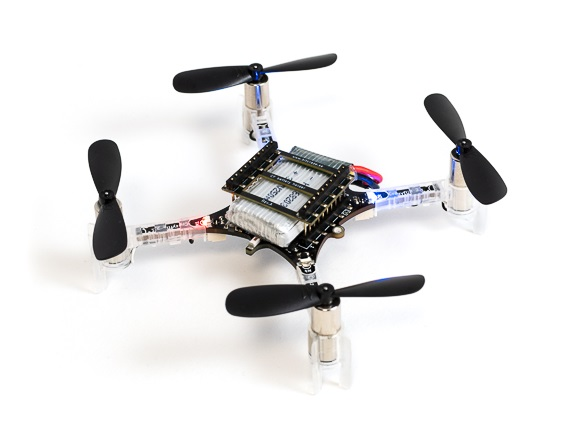
\includegraphics[width=.6\linewidth]{NN/drone_real.jpg}
\end{figure}
%
Here we consider another benchmark which is based on a reinforcement learning
environment: autonomous drone control. In particular, we consider the 
problem of making a drone take off and hover at a chosen altitude. Our motivation 
for dealing with a robotics framework is twofold: first, the control problems
arising in robotics are more and more relevant in the real world scenario; drones
and unmanned agents in general are being employed in several tasks that require
a high confidence in the agent. Second, using the Soft Actor-Critic architecture 
we are able to employ reasonable-sized network architectures for the agent that 
we are able to verify, and we delegate the more complex tasks to the critic which 
is not required to be certified.

We focused on building a modular setup for the generation of benchmarks using well-maintained
and stable resources to be able to easily extend it to new case studies and network 
architectures. In particular, we leveraged:
%
\begin{itemize}
	\item \gym\footnote{https://github.com/openai/gym}: an open source Python 
	library providing a standard API for communication between reinforcement 
	learning algorithms and environments.
	\item \stableb\footnote{https://github.com/DLR-RM/stable-baselines3}: an 
	open source training framework providing scripts for training and evaluating 
	RL agents using standard state-of-the-art algorithms.
	\item \pybullet\footnote{https://pybullet.org/}: an open source physics 
	simulator for robotics and reinforcement learning.
	\item \drones\footnote{https://github.com/utiasDSL/gym-pybullet-drones}: an 
	open source \gym-stile environment supporting the definition of various 
	learning tasks on the control of one or more quadcopters.
\end{itemize}
%
Using these open source resources we greatly simplified the complexity of our 
setup and we were able to directly train the network of interest in the environment 
corresponding to our case study with the chosen state-of-the-art RL algorithm.
In Figure~\ref{fig:drone} we show the quadcopter model of choice,
which was the default one proposed in \drones{} (Bitcraze's Crazyflie 2.x).
To evaluate our algorithms we built the experimental setup detailed in the following.
%
\paragraph{RL setup.} The reinforcement learning setup we used to train 
our model was based on the one proposed by~\cite{DBLP:conf/iros/PaneratiZZXPS21}: 
in particular, we leveraged their \textsc{HoverAviary} environment, together with 
the \stableb{} implementation of the Soft Actor-Critic (SAC) algorithm,
to train our neural networks of interest. We chose this algorithm because
it is more stable than traditional actor-critic algorithms, but it still makes
use of two different networks: the \textit{actor} to learn a
policy and the \textit{critic} to approximate the optimal value
function. Because of this, it is possible to learn a relatively small
actor network, which is then subject to verification, while the critic
network can be as complex as the task requires without impacting on
the verification performances since only the actor network is relevant
for this purpose. 
The hyperparameters chosen for the SAC algorithm were the default ones proposed 
by \stableb{} except for the network architectures of the actor and the critic: 
in particular, for the critic we chose a fixed architecture with four hidden layers 
with $512, 256, 128, 64$ neurons, respectively, each followed by a ReLU layer, 
whereas for the actor we considered the eight different architectures presented in
Table~\ref{tab:ac-arch}.
%
\begin{table}[t]
	\caption{\label{tab:ac-arch}Actor network architectures used in our 
		experimental evaluation, arranged in two (\textit{AC1} to \textit{AC4}) 
		or three (\textit{AC5} to \textit{AC8}) hidden layers. The size of layers, 
		i.e., the number of neurons in each layer, is detailed in column 
		\textbf{No. of neurons}. Each hidden layer is followed by a ReLU layer.}
	\setlength{\tabcolsep}{15.5pt}
	\centering
	%\begin{tabular}{c c c}
	\begin{tabular}{l c r}
		\toprule
		\textbf{Architecture} & \textbf{Network ID} & \textbf{No. of neurons} \\
		\midrule
		\multirow{4}{*}{\textbf{Two layers}} & \textit{AC1} & 32, 16 \\
		& \textit{AC2} & 64, 32 \\
		& \textit{AC3} & 128, 64 \\
		& \textit{AC4} & 256, 128 \\
		\midrule
		\multirow{4}{*}{\textbf{Three layers}} & \textit{AC5} & 32, 16, 8 \\
		& \textit{AC6} & 64, 32, 16 \\
		& \textit{AC7} & 128, 64, 32 \\
		& \textit{AC8} & 256, 128, 64 \\
		\bottomrule
		\bigskip
	\end{tabular}
\end{table}

The observation type considered was the kinematic information (pose, linear and angular 
velocities) of the quadcopter, and the action type was the revolutions per minute 
(RPMs) applied to all the four rotors of the drone (similarly to what is done in
the experimental evaluation of~\cite{DBLP:conf/iros/PaneratiZZXPS21}).
All the actor models considered in our experiment were trained 
for 50000 steps and, at the end of the training process, the version
of the actor model 
presenting the best mean reward in an evaluation environment was chosen.
%
%
\paragraph{Verification setup.} The verification task we consider in our 
experiments is an analysis of the local robustness of our actor model with respect to 
small variations of the input, which could be interpreted as small noise on the 
sensors providing the input signal. Formally we consider the following assumption:
%
\begin{equation}
	\forall \varepsilon, x_0: \quad |x - x_0|_\infty \leq \varepsilon \quad \rightarrow \quad \nu(x_0) - \delta \leq \nu(x) \leq \nu(x_0) + \delta
	\label{eq:local-robustness}
\end{equation}
%
where $x_0$ is a specific input vector for the network $\nu$, and $\varepsilon$ and 
$\delta$ are scalar values representing the maximum noise on the input and the 
corresponding maximum output deviation, respectively. Our aim is to determine the 
values of $\delta$ corresponding to fixed values of $\varepsilon$ and $x_0$ for all 
the actors presented in Table~\ref{tab:ac-arch}.
The encoding of this verification task is straightforward in \nevertwo{}: we only need 
to define as input star the convex polytope defined by the constraints corresponding 
to $|x - x_0|_\infty \leq \varepsilon$ and then propagate it in our abstract network, 
applying the abstract transformer presented in Section~\ref{sec:relu_abst}, to 
obtain the abstract output set, whose stars can be easily analyzed to compute the 
reachable bounds of the output and, as a direct consequence, the maximum value of 
$\delta$. In the experiments we evaluated our complete, over-approximate and mixed 
algorithms: in particular, in our mixed algorithm we considered the case in which 
a single neuron is refined for each ReLU layer. We also considered two different 
values ($0.1$, $0.01$) for $\varepsilon$.
\\\\
Our experimental setup is available online in the public repository of
\pynever\footnote{https://github.com/NeVerTools/pyNeVer/tree/main/examples/submissions/IEEEAccess2023}, 
and the experiments herewith presented can be easily replicated.
The experiments were run on a machine with 2 Intel Xeon Gold 6432 CPUs and 128 GB of DDR4 RAM.
%